\documentclass[journal,twoside,web]{ieeecolor}
\usepackage{generic}
\usepackage{cite}
\usepackage{amsmath,amssymb,amsfonts}
\usepackage{algorithmic}
\usepackage{graphicx}
\usepackage{textcomp}
\usepackage{color}
\usepackage{soul}
\usepackage{booktabs} % 표를 더 깔끔하게 만들기 위한 패키지
\usepackage{tabularx} % 표의 너비 조정을 위한 패키지
\usepackage{hyphenat}
\usepackage{hyperref}
\usepackage{ulem}
\usepackage{soul}
\usepackage{booktabs}
\usepackage{array}
\def\BibTeX{{\rm B\kern-.05em{\sc i\kern-.025em b}\kern-.08em
    T\kern-.1667em\lower.7ex\hbox{E}\kern-.125emX}}
\markboth{\journalname, VOL. XX, NO. XX, XXXX 20XX}
{Author \MakeLowercase{\textit{et al.}}: Preparation of Papers for IEEE TRANSACTIONS and JOURNALS (February 2017)}
\begin{document}
\IEEEaftertitletext{\vspace{-1cm}} % 제목 밑 공간
\title{Time-step-free Physics-Based Modeling of Retention Loss in Cryogenic 3-D NAND Flash}\author{Myung Jin, Haechan Choi, and Hyungcheol Shin, \IEEEmembership{Senior Member, IEEE}
\thanks{This paragraph of the first footnote will contain the date on 
which you submitted your paper for review. (\textit{Corresponding Author: Myung Jin; Hyungcheol Shin.}) }
\thanks{Myung Jin and Haechan Choi are with the Department of Electrical and Computer Engineering, Seoul National University, Seoul 08826, South Korea (e-mail: gsjb1028@snu.ac.kr).}
\thanks{Hyungcheol Shin is with the Department of Electrical and Computer Engineering, Seoul National University, Seoul 08826, South Korea, and also with Integra Semiconductor, Ltd. (e-mail: hcshin@snu.ac.kr).}}

\maketitle
% \vspace{-1cm}


\begin{abstract}
We propose a time-step-free physics-based model for detrapping-induced retention loss in cryogenic 3-D NAND flash memory.
By solving the first-order autonomous detrapping equation in closed form, the proposed model directly evaluates $\Delta V_\text{th}(t)$ from the initially programmed trapped charge distribution without transient time stepping.
For a fixed number of targeted retention times, the computational cost is independent of the final physical retention time, enabling efficient short- and long-term retention prediction.
The validation was done by calibrated TCAD simulation to cryogenic condition, which have been achieved by $\sigma_n \rightarrow 0$ due to limitation of TCAD in cryogenic simulation.
Time-step-free model showed good match to the TCAD simulation.
\end{abstract}

\begin{IEEEkeywords}
time-step-free modeling, autonomous ODE, detrapping, 3-D NAND flash memory, retention loss modeling
\end{IEEEkeywords}

\section{Introduction}
\label{sec:introduction}
\IEEEPARstart{T}{here} rapid increase in data storage demand, driven by emerging computing technologies such as artificial intelligence (AI) and high-performance computing (HPC), has raised significant concerns about the reliability of 3-D NAND flash memories, particularly regarding retention loss~\cite{agoda}.

As storage capacity per cell increases, ensuring long-term stability of each bit’s threshold voltage distribution over time scales from days to years becomes increasingly critical.
Moreover, prior works have shown that charge detrapping can still occur at cryogenic temperatures~\cite{Refaldi.IRPS2025}, supporting models that treat detrapping as largely temperature independent~\cite{Jin.TED2025}.

In this study, a time-step-free physics-based model is developed for retention loss based on tunneling emission mechanisms in 3-D NAND flash memory.
The proposed simulation framework uses the initially programmed trapped charge distribution as input and enables highly efficient computation by using closed-form solution of the autonomous detrapping equation, eliminating sequential transient time stepping.


\section{Modeling}

This section presents the modeling framework for time-step-free simulation of retention loss.
First, a cylindrical Poisson solution is derived for the oxide–nitride–oxide (O/N/O) gate stack, incorporating quantized multiple layers within the charge trap nitride (CTN) layer.
After obtaining the detailed Poisson solution for these discretized layers, the threshold voltage shift ($\Delta V_\mathrm{th}$) is calculated using an optimized numerical scheme.
Finally, based on previous studies of detrapping-induced emission rates~\cite{Jin.TED2025}, an autonomous equation governing retention loss behavior is proposed.

\subsection{Detailed Poisson Solution}

An electrical potential distribution obtained from the cylindrical Poisson equation for discretized layers in the ONO structure can be expressed as follows~\cite{Jin.TED2025,Amoroso.TED}.
\begin{equation}
\begin{cases}
V_\mathrm{Si}(r_\text{Si}) = V_\mathrm{ch} \\
V_\mathrm{TOX}(r) = V_\mathrm{ch} + \frac{K_\mathrm{TOX}}{\epsilon_\mathrm{TOX}}\ln{\frac{r}{r_\text{Si}}} \\
V_{\mathrm{CTN},i}(r) = V_{\mathrm{CTN},i-1} (r_{i-1}) + \frac{K_{i}}{\epsilon_\mathrm{CTN}} \ln{\frac{r}{r_{i-1}}} \\
V_\mathrm{BOX}(r) = V_{\mathrm{CTN},N} (r_{N}) + \frac{K_\mathrm{BOX}}{\epsilon_\mathrm{BOX}}\ln{\frac{r}{r_{N}}} \\
V_\mathrm{BOX}(r_\mathrm{BOX}) = V_\text{G}
\end{cases}
\end{equation}
\noindent where $i=1$–$N$ denotes the index of each discretized slice of the CTN layer in the radial direction, and $N$ is the total number of radial partitions.

Solving $\mathbf{x}$ vector can calculate the total $N+2$ potential parameters.

\begin{equation}
\mathbf{x} = \begin{bmatrix}
K_{TOX} & K_1 & \cdots & K_N & K_{BOX} \\
\end{bmatrix} ^\top
\end{equation}

\begin{equation}
A\mathbf{x} = \mathbf{b}
\end{equation}

Matrix $\mathrm{A}$ and vector $\mathbf{b}$ are constructed by enforcing a total of $N+1$ transverse electric field continuity conditions ($\epsilon_1 \mathcal{E}_1 = \epsilon_2 \mathcal{E}_2$) together with an additional boundary condition defined by reference potential.

\begin{equation}
    \label{A}
A =
\begin{bmatrix}
1 & -1 & 0  & \cdots & 0 & 0 \\
0 & 1 & -1 & \cdots & 0 & 0 \\
\vdots & & & \ddots  & & \vdots \\
0 & 0 & 0 & \cdots & 1 & -1 \\
\frac{2\pi}{C_{\mathrm{TOX}}} & \frac{2\pi}{C_1} & \frac{2\pi}{C_2} &
\cdots & \frac{2\pi}{C_N} & \frac{2\pi}{C_{\mathrm{BOX}}}
\end{bmatrix}
\end{equation}


\begin{equation}
    \label{b}
\mathbf{b} =
\begin{bmatrix}
\frac{\Delta Q_0}{2\pi} &
\frac{\Delta Q_1}{2\pi} &
\cdots &
\frac{\Delta Q_N}{2\pi} &
\Delta V
\end{bmatrix} ^\top
\end{equation}

\begin{equation}
    \label{Delta Q}
    \Delta Q_i = \pi r_i^2\left(n_{t,i} - n_{t,i-1}\right)
\end{equation}

\begin{equation}
    \label{Delta V}
\Delta V = (V_\text{G} - V_\text{ch}) - \sum_{i=1}^{N} \frac{q n_{t,i}}{4 \epsilon_\mathrm{CTN}}\left(r_i^2 - r_{i-1}^2\right)
\end{equation}

$C_\mathrm{TOX}$, $C_i$, and $C_\mathrm{BOX}$ in \eqref{A} denote the capacitances of each cylindrical layer, as illustrated in Fig. 1(c).
$\Delta Q_i$ in \eqref{b} represents the charge component associated with the cylindrical shell at radius $r_i$, which can be superpositioned as $Q=\sum \Delta Q_i$ as demonstrated on Fig. 1(d).
Furthermore, \eqref{b} indicates that $\mathbf{b}(\Delta Q_i, V_\text{G} - V_\text{ch})$ varies with the trapped charge distribution and the applied voltage conditions.

\begin{figure}[!t]
    \centering
    
\includegraphics[width=\columnwidth]{fig1.png}
    \caption{(a) shows a radial slice of 3-D NAND flash memory, 
    (b) shows the programmed trapped charge distribution, 
    (c) shows capacitance and node charge representation,
    and (d) shows the visualization of $\Delta Q_i$ for each node.}
    \label{fig1}
\end{figure}


\subsection{Q - $\Delta V_\text{th}$ Relation}
For the $\Delta V_\text{th}$ calculation, the gate voltage difference required to maintain equal channel field conditions must be determined~\cite{Amoroso.TED,Jin.TED2025}.
\begin{equation}
    F_\mathrm{TOX}(r_\text{Si}) = \frac{K_\mathrm{TOX}}{\epsilon_\mathrm{TOX}} \frac{1}{r_\text{Si}}
\end{equation}

To achieve equal channel field conditions, the same $K_\mathrm{TOX}$ value under the given conditions must be established.  
By Cramer's rule, the $K_\mathrm{TOX}$ parameter can be solved through determinant calculation.
\begin{equation}
    K_\mathrm{TOX} = \frac{\det \left[A_{\mathbf{b}(\Delta Q_i,\Delta V_\text{th})}\right]}{ \det A}
\end{equation}

\noindent where notation $A_{\mathbf{b}(\Delta Q_i,\Delta V_\text{th})}$ stands for $1^\text{st}$ column of matrix $A$ replaced with vector $\mathbf{b}(\Delta Q_i , \Delta V_\text{th})$.

Therefore, $\Delta V_\text{th}$ can be solved easily by using the property of multilinearity.

\begin{equation}
    \label{double.Det}
    \det \left[A_{\mathbf{b}(0,\Delta V_\text{th})}\right] = -\Delta V_\text{th}  = \det \left[A_{\mathbf{b}(\Delta Q_i,0)}\right]
\end{equation}

\begin{equation}
    \therefore \Delta V_\text{th} = -\det \left[A_{\mathbf{b}(\Delta Q_i,0)}\right]
\end{equation}

The threshold voltage difference can be calculated with single determinant computation with initially programmed trapped charge distribution is given as Fig.~\ref{fig2}(b).

\begin{figure}[t!]
    \centering
    
\includegraphics[width=\columnwidth]{fig2.png}
    \caption{(a) The band diagram with barrier notations where detrapping of trapped electron occurs,
    (b) a detail programmed trapped charge distribution after program operation~\cite{C.Lee.JJAP2026, H.Choi.TED2024}, 
    and (c) TCAD parameter deck and used trap profile within the simulation~\cite{Jin.TED2025,Jo.TED2025,Verreck.IEDM}.}
    \label{fig2}
\end{figure}


\subsection{Time-step-free Detrapping Modeling}
With the given initial conditions, an autonomous equation is established for each cell, divided by radial position and trap depth.
\begin{equation}
    \frac{d}{dt}{n_t}(r, E_t, t) = -(e_\text{ch} + e_\text{WL}){n_t}(r, E_t, t)
\end{equation}

Then, detrapping relation can be express as following autonomous ODE solution.
\begin{equation}
    n_t(r, E_t, t) = \sum_r \sum_{E_t}n_{t0}(r, E_t) \exp (-(e_\text{ch} + e_\text{WL})t)
    \label{autonomousSoluation}
\end{equation}
% \noindent for hole concentration ($h_t$) vice versa.

The emission rate for trapped electron can be computed as following equations based on a previous study \cite{Jin.TED2025}.
\begin{equation}
    e = \nu \times \left|TC\right|
\end{equation}
\begin{equation}
    \nu = \frac{2 \pi}{\hbar} \left|E_t\right|^2 V_\text{trap} \cdot \frac{m_0\sqrt{2m^*}}{\pi^2 \hbar^3}\sqrt{E-E_\text{trap}}
\end{equation}
\begin{equation}
    \left|TC\right| = \prod \exp{\left(-\frac{4\sqrt{2m^*}}{3\hbar q} \frac{\Phi_H^{1.5} - \Phi_L^{1.5}}{F}\right)}
\end{equation}

\noindent for both channel and wordline directions as demonstrated in Fig.~\ref{fig2}(a).

This autonomous detrapping modeling equation (\ref{autonomousSoluation}) is the key relation that enables a simulation to directly compute the result at a specific time once initially programmed trapped charge distribution is specified.
Therefore, for a fixed spatial/energy discretization and a fixed number of evaluated retention times, the computational cost is governed by the number of trap bins rather than by the final physical retention time.

\section{Simulation and Result}


\begin{figure}
    \centering
    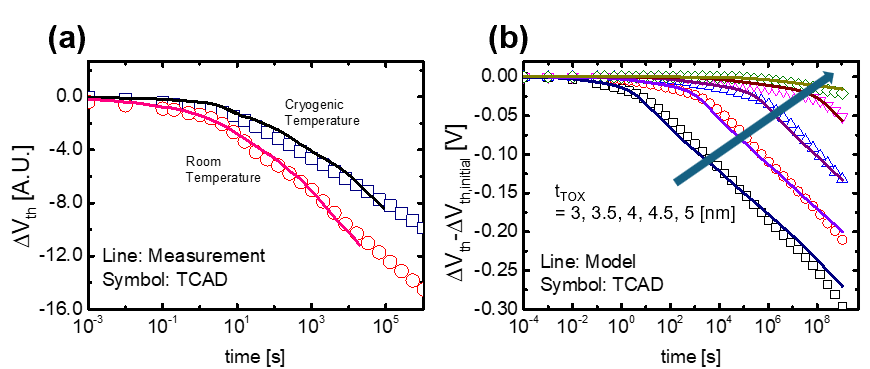
\includegraphics[width=\columnwidth]{fig3.png}
    \caption{(a) The TCAD simulation calibration with the measurement from previous study~\cite{Refaldi.IRPS2025}.
    (b) A detail detrapping curve variation over time with $t_\text{TOX}$ from 3~nm to 5~nm.}
    \label{fig3}
\end{figure}

According to Refaldi et.al~\cite{Refaldi.IRPS2025}, cryogenic conditions enable the detrapping component to be isolated from retention loss.
However, direct TCAD simulation at cryogenic temperature below 4.2~K condition did not converge reliably in our setup.
Therefore, to emulate cryogenic conditions during retention operation within the TCAD framework, the capture cross-section was adjusted to an extremely low value ($\sigma_\mathrm{n} \rightarrow 0$) only during retention. 
This manipulation suppresses thermal electron transitions between trapped and conduction states within the CTN layer, while maintaining physical consistency in other mechanisms~\cite{TCADmanual.2022}.

The TCAD deck shown in Fig.~\ref{fig2}(c) was calibrated by matching the retention time scale of the measurement in previous study~\cite{Refaldi.IRPS2025}.
Since $\Delta V_\text{th}$ in~\cite{Refaldi.IRPS2025} is reported in arbitrary units, the calibration was done by matching time scale only.
Program operation was performed by single $1~\mu s$ pulse and calibrated to obtain $\Delta V_\text{th} = 1.8~V$.

To properly focus on the detrapping effect from the CTN layer, bandgap-engineered processes were neglected and program operation was perfomed with fresh cell.
Lateral migration retention loss was ignored by selecting neighboring data pattern~\cite{Chou.IEDM2023}.

The model validation is performed using Synopsys TCAD simulations calibrated against previous retention modeling studies~\cite{Jo.TED2025, Jin.TED2025}. 
The variation of the $t_{ox}$ showed the most dominancy in detrapping time transient curve.
In Fig.~\ref{fig3}(b), $t_{ox}$ from 3~nm to 5~nm for both TCAD simulation and the model were perfomed, showing good match with each other.

Table~\ref{MethodComparisons} shows the comparison between TCAD and the model.
The table shows how much computation time and resource efficiency could be improved through the autonomous model.
Since autonomous model's computation time is independent from sequential time step, can be adopted to both short and long term retention operation based on given physical time.

\begin{table}[t]
\caption{Comparison between a TCAD and the autonomous model}
\label{MethodComparisons}
\centering
\begin{tabular}{lcc}
\toprule
Property & TCAD & Time-step-free model\\
\midrule
\shortstack[l]{Temporal treatment\\{}} & \shortstack[l]{sequential time stepping\\{}} & \shortstack[l]{closed-form evaluation\\of eq (\ref{autonomousSoluation})}\\
\shortstack[l]{Dependence on\\final physical time\\{}} & {\shortstack[l]{Runtime increases with\\the final retention time\\{}}}& \shortstack[l]{Runtime independent of\\final physical time} \\
\shortstack[l]{Run Time (s)\\(average of Fig.~\ref{fig3}(b))} & \shortstack[l]{27483\\{}} & \shortstack[l]{3.926\\{}} \\
\bottomrule
\end{tabular}
\end{table}



\section{Conclusion}
This study presents a time-step-free physics-based modeling for retention loss due to detrapping of trapped electrons. 
the novelty of time-step-free modeling is demonstrated through significant computational optimization, achieving runtime independent of final physical time.
Additionally, compared to TCAD simulations calibrated with physical parameters from various prior studies, the proposed model demonstrates good match with TCAD simulation within extremely short timeframe. 

\begin{thebibliography}{00}

\bibitem{agoda} A. Goda, K. K. Muchherla, and P. Feeley, "Reliability of 3D NAND Flash for Future Storage Systems (Invited)," 2023 IEEE International Reliability Physics Symposium (IRPS), Monterey, CA, USA, 2023, pp. 1-10, doi: 10.1109/IRPS48203.2023.10118280.

\bibitem{Refaldi.IRPS2025} D. G. Refaldi, G. Malavena, L. Chiavarone, N. Gagliazzi, A. S. Spinelli, and C. M. Compagnoni, "Cryogenic Investigation of Vertical Charge Loss in 3D NAND Flash Memories," 2025 IEEE International Reliability Physics Symposium (IRPS), Monterey, CA, USA, 2025, pp. 1-7, doi: 10.1109/IRPS48204.2025.10983672.

\bibitem{Jin.TED2025} M. Jin and H. Shin, "Modeling Attempt-to-Escape Frequency: Tunneling Emission of Trapped Electrons in Tunneling Oxides of 3-D NAND Flash Memory," in IEEE Transactions on Electron Devices, vol. 72, no. 9, pp. 4884-4889, Sept. 2025, doi: 10.1109/TED.2025.3589340.

\bibitem{Amoroso.TED} S. M. Amoroso, C. Monzio Compagnoni, A. Mauri, A. Maconi, A. S. Spinelli, and A. L. Lacaita, "Semi-Analytical Model for the Transient Operation of Gate-All-Around Charge-Trap Memories," in IEEE Transactions on Electron Devices, vol. 58, no. 9, pp. 3116-3123, Sept. 2011, doi: 10.1109/TED.2011.2159010.

\bibitem{C.Lee.JJAP2026} C. Lee and H. Shin, "Investigation and modeling of vertical redistribution in charge-trap-based 3D NAND Flash memory." Japanese Journal of Applied Physics 65.1 (2026): 011004, doi: 10.35848/1347-4065/ae3161

\bibitem{H.Choi.TED2024} H. Choi, J. Yoo, and H. Shin, "A New Physical Model for Program Transients of Cylindrical Charge-Trap-Based NAND Flash Memories," in IEEE Transactions on Electron Devices, vol. 71, no. 4, pp. 2386-2392, April 2024, doi: 10.1109/TED.2024.3364587.

\bibitem{Verreck.IEDM} D. Verreck, A. Arreghini, F.Schanovsky, G. Rzepa, Z. Stanojevic, F. Mitterbauer, C. Kernstrock, O. Baumgartner, M. Karner, G. Van den bosch, and M. Rosmeulen, "Understanding the ISPP Slope in Charge Trap Flash Memory and its Impact on 3-D NAND Scaling," 2021 IEEE International Electron Devices Meeting (IEDM), San Francisco, CA, USA, 2021, pp. 1-4, doi: 10.1109/IEDM19574.2021.9720506.

\bibitem{Jo.TED2025} I. Han and H. Shin, "Machine Learning-Based Investigation of Temperature Effects on Lateral Migration in 3-D nand Flash Memory," in IEEE Transactions on Electron Devices, vol. 73, no. 5, pp. 2747-2753, May 2026, doi: 10.1109/TED.2026.3673641.

\bibitem{TCADmanual.2022} TCAD Sentaurus Device User Guide Version 2022, Synopsys, Mountain View, CA, USA, Mar. 2022.

\bibitem{Chou.IEDM2023} Y. L. Chou, C. C. Lu, W. J. Tsai, T. C. Lu, K. C. Chen, and C. Y. Lu, "A Target-Read Retry Scheme for 3D Charge Trap NAND Flash Memory," 2023 International Electron Devices Meeting (IEDM), San Francisco, CA, USA, 2023, pp. 1-4, doi: 10.1109/IEDM45741.2023.10413738.


\end{thebibliography}


\end{document}
